% Template for PLoS
% Version 1.0 January 2009
%
% To compile to pdf, run:
% latex plos.template
% bibtex plos.template
% latex plos.template
% latex plos.template
% dvipdf plos.template

\documentclass[10pt]{article}

% amsmath package, useful for mathematical formulas
\usepackage{amsmath}
% amssymb package, useful for mathematical symbols
\usepackage{amssymb}
\usepackage{url}
% graphicx package, useful for including eps and pdf graphics
% include graphics with the command \includegraphics
\usepackage{graphicx}

% cite package, to clean up citations in the main text. Do not remove.
\usepackage{cite}

\usepackage{color} 

% Use doublespacing - comment out for single spacing
%\usepackage{setspace} 
%\doublespacing


% Text layout
\topmargin 0.0cm
\oddsidemargin 0.5cm
\evensidemargin 0.5cm
\textwidth 16cm 
\textheight 21cm

% Bold the 'Figure #' in the caption and separate it with a period
% Captions will be left justified
\usepackage[labelfont=bf,labelsep=period,justification=raggedright]{caption}

% Use the PLoS provided bibtex style
\bibliographystyle{plos2009}

% Remove brackets from numbering in List of References
\makeatletter
\renewcommand{\@biblabel}[1]{\quad#1.}
\makeatother


% Leave date blank
\date{}

\pagestyle{myheadings}
%% ** EDIT HERE **


%% ** EDIT HERE **
%% PLEASE INCLUDE ALL MACROS BELOW

%% END MACROS SECTION

\begin{document}

% Title must be 150 characters or less
\begin{flushleft}
{\Large
\textbf{DIY Decoding of Human Activity from Low Quality Brainwaves}
}
% Insert Author names, affiliations and corresponding author email.
\\
Thomas Maillart$^{1}$, 
John Chuang$^{1}$
%Author3$^{3,\ast}$
\\
\bf{1} School of Information, UC Berkeley, Berkeley, CA, USA
$\ast$ E-mail: Corresponding maillart@berkeley.edu
\end{flushleft}

% Please keep the abstract between 250 and 300 words
\begin{abstract}
At the age of online information abundance, the human capacity to retain knowledge is largely limited by the time and the attention required to read text, watch videos, listen to podcasts. For written information, rapid serial visual presentation (RSVP) helps greatly save time with similar levels of text understanding, compared with traditional reading. However, RSVP does not account for attention. We present a simple hybrid brain-computer interface (BCI) that controls in real-time the speed of reading by measuring the instant level of higher cognitive brain activity. Electroencephalogram (EEG) signal is acquired with a single channel consumer-grade headset and analyzed in the frequency domain. The pace of word display is controlled by a measure brainwave entropy. We have conducted a controlled experiment with 50 subjects with three distinct treatments, and we show that brain-controlled speed-reading increases the speed and the understanding of texts by subjects.
\end{abstract}
% Please keep the Author Summary between 150 and 200 words
% Use first person. PLoS ONE authors please skip this step. 
% Author Summary not valid for PLoS ONE submissions.   
%\section*{Author Summary}

\section{Introduction}

\section{Method}

\subsection{Brain Speed Reader}

{\bf describe the brain control system}

\begin{enumerate}
  \item capture brainwaves for 1 second
  \item compute power spectrum
  \item compute normalized entropy
  \item update display speed ({\bf trick of the moving average to be described here})
\end{enumerate}


\subsection{Experimental Protocol}


\begin{enumerate}
  \item Constant Rate
  %\item Randomly Varying Text : AR(1) $\rigtharrow$ AR1(n,baseline,baseline/2,0.5,sigma=std) AR1 formula : $c + phi * X[-1] + np.random.normal(scale=sigma)$
  %\item Brain Speed Reader : (i) compute entropy $S$ at t, (ii) normalize $S$ as $S_{norm} = (S- \langle S \rangle) / \sigma_S$, with $\langle S \rangle$ and $\sigma_S$ computed over the last XX values of entropy, (iii) compute a new speed as $v(t+1) = v(t)\cdot(1-0.2\sdot S_{norm})$
\end{enumerate}


\subsection{Measuring Text Complexity}

ATOS  ( ref: Michael Milone,The Development of ATOS, The Renaissance Readability Formula, p10 (2010) \url{http://doc.renlearn.com/KMNet/R004250827GJ11C4.pdf}

\begin{itemize}
  \item Words per sentence
  \item Average grade level of words ( which class grade the word is first seen)
  \item Characters per word
\end{itemize}


$ATOS Rasch Difficulty Formula = -8.54 + 1.95 * Ln(AvgWords) + .46 * AvgGrad100 + 1.74 * Ln(AvgChar)$

Adjustment for books with less than 500 words

$BLGL for Books With Fewer Than 500 Words = .004 * Book Length + 0.4$


Table detailing texts : \url{https://docs.google.com/spreadsheets/d/1uwkoToM-p3UFrd0U_1vOX4eBJsmYuPVYVhvhsZ8Y5Nc/edit#gid=0}




%\begin{itemize}
%  \item {\bf text 0 (adapted from Coming of Age in Samoa, Margaret Mead, 1928
%)}:   $ATOS=9.5$,  $word~count = 421$
%  \item {\bf Text 1  (adapted from The Warden, Anthony Trollope, 1855)} : $ATOS=8.3$, $word~count = 563$
%  \item {\bf Text 2  (adapted from The Mayor of Casterbridge, Thomas Hardy, 1886) } : $ATOS=10.2$, $word~count = 831$
%  \item {\bf Text 3 (Adapted from: The Social Function of Science, John D Bernal (1939))} : $ATOS=11.9$, $word~count = 421$
%\end{itemize}



\section{Results}
\label{results}


For $17$ over $21$ participants, the RSVP rate was characterized by a balanced joint probability of {\it rate change x word size frequency} in treatment (ii) and (iii) (Fig. 2a). Long words triggered the largest change of entropy (resp. rate), while words smaller than the average size ( $< 5.5$ characters) were associated with reverse entropy (resp. rate) change (Fig. 2b, 2c).\\

Despite the large variation of entropy, texts could be decoded by matching the sequence of entropy measures (associated with each word) with the unique sequence of word lengths (Fig 3). Our results did not require preliminary identification of participants, and the success rate was 27.4\%, roughly 11\% above chance (i.e., $1/6 \approx 16.67\%$), when considering the first 300 words of each text.



\begin{itemize}
  \item performance*, perceived comfort and control as a function of treatment 
  \item for brain speed reader treatment:  performance*, perceived comfort and control as a function $X_0$, $alpha$
\end{itemize}

*performance means either {\bf conceptual} (understanding the meaning), {\bf conceptual-memory} (recalling characters) or {\bf memory} (recalling some words).




%\input{../sections/data}
%\input{../sections/dynamicsAnalysis}
%\input{../sections/tailAnalysis}
%\section{Discussion}
\label{discussion}
Recognizing the importance of reading more in less time, while avoiding multi-tasking, we have put to the test the {\it brain speed reader}, a brain-computer interface (BCI) implementing a rate varying rapid serial visual presentation (RSVP) of text words. We have found that a majority of users who participated in our study could control the brain speed reader. Furthermore, we found that roughly half of participants could self-regulate with two opposite control mechanisms ({\it bsr+} and {\it bsr-}). The achievement of self-regulation is negatively influenced by age, text length, topic familiarity and speed reading comfort. Self-regulation achievement (stability) is however highly positively correlated with reading pleasure. Capacity to provide a meaningful text summary {\it ex-post} (the best way to test for text comprehension) is also positively associated with stability, yet in a weakly significant way.

Our results show that the brain speed reader is an adequate technology to foster fast knowledge integration in a world of abundant information and endless news feeds, while at the same time helping preventing multi-tasking. The design implements self-regulation neurofeedback as a way to ensure that users concentrate on reading the text: If the user does not or cannot concentrate, the RSVP rate will drift towards very slow (resp. fast) word display rates. Multi-tasking is discouraged by design, and reading speed is doubled compared to normal reading.

Self-regulation neurofeedback stems from the capacity by the brain to train and adapt its wave modulations in order to perform specific tasks better \cite{piano_neurofeedback}, or to reach desired mental states \cite{neurofeedback_meditation}.  As a special kind of neurofeedback BCI, the brain speed reader may be help remediate reading disabilities or difficulties associated with a lack of concentration capabilities, which is one consequence of multi-tasking. Because the brain speed reader (BSR) does not require prior calibration, training and use occur concomitantly: Either the user achieves self-regulation quickly and then {\it uses} BSR, or she remains in training mode until she reaches self-regulation. In our experiment, we have set very large boundary for slowest (resp. fastest) RSVP rate to make sure that subjects who reach the boundaries effectively failed achieving self-regulation. In training mode, these RSVP rate boundaries may be tuned and personalized to ensure that the user can reach a compromise between attempts to achieve self-regulation and still reading fast with pleasure while training. While we have not tested medical applications for the brain speed reader, it may help users suffering from dyslexia or attention disorder and hyperactivity disorders (ADHD) improve their reading and their attention.

\subsection{Limitations}
The version of the brain speed reader presented here is a first attempt to harness self-regulated neurofeedback for the sake of upgrading the reading experience to arising challenges in society, such as tackling the abundance of natural language- written information while reducing multi-tasking. Although our first experiment show encouraging results, we have come up with the simplest possible implementation and experimental protocol. A number of outstanding questions remain and deserve further work, starting with the hardware we used. Neurofeedback most often involves a limited number of EEG electrodes, but typically of higher quality and on other positions in the 10-20 system. One may want to experiment with a variety of electrode quality, number, and positions to elicit a better hardware configuration.

Our study bears a number of limitations regarding comprehension and memory. We did not find a significant difference of comprehension between RSVP speed read at constant rate versus {\it bsr+} and {\it bsr-} treatments. We find a slight comprehension improvement when users achieve more stable self-regulation, but this result need further validation, presumably with a larger data set. We have also not measured how comprehension and word recall are diminished (resp. increased) as reading speed doubles, i.e., when comparing brain speed reading and reading text normally. Previous research suggests that comprehension is diminished by constant RSVP rate speed reading \cite{kujala2007phase}, although it remains the same or is slightly improved for people with reading disabilities. Further investigation is required to better elicit how self-regulation stability influences comprehension and word recall

We shall also investigate why some participants could not achieve self-regulation: It remains unclear if they had indeed to train further before making it right, or if the BSR parameters we chose [initial RSVP rate $X(t=0) = 125$ ms/word and $|\alpha| = 0.005$] may only be suitable for a subset of the population, and may require further adaptation. Similarly, we have no information on the time it takes to learn given that the user could not achieve self-regulation at once. We chose $X(t=0) = 125$ ms/word as the starting RSVP rate, which is also the value known to be most comfortable on average to people who read with RSVP. To further understand and validate the self-regulation mechanism, it would be desirable to perform additional investigations with a variety of starting rates. Our hypothesis is that within a yet unknown RSVP rate range, users capable of self-regulation can stabilize the rate, while beyond some limits it is impossible to control the brain speed reader, in particular when the presentation speed is high. It also remains to be seen if users tend to stabilize the rate close to 125ms/word on average, even if the initial RSVP rate is smaller (resp. larger).

Even though there is no need for preliminary {\it ad-hoc} calibration to use the brain speed reader, learning still occurs ``on the fly", with several advantages as already mentioned above. It would nevertheless be desirable to better understand how the user transitions from {\it learning} to {\it using}. This has implications for more elaborate and personalized UX design.

Finally, we found that text length has a negative effect on self-regulation stability (roughly one unit per 1300 words as shown in Table \ref{tab:reg}). This is a concern because the brain speed reader is supposed to let users avoid multi-tasking to concentrate on a single task instead. Here, it appears that if the task lasts too long, then self-regulation undergo changes of regime and reduced stability. This suggests that either BSR is suited for {\it long but not that long tasks} and/or there is another factor involving learning how to keep self-regulation highly stable over long tasks. This is has further implications on comprehension and memory, which need to be further addressed.

\subsection{Beyond speed reading}
Here, we have designed and tested brain-computer interface (BCI), which helps seamlessly control the parsing rate of a coherent sequence of a words as visual stimuli. The same time varying rate RSVP coupled with a neurofeedback BCI may be used beyond reading. It could apply similarly to cartoons, video or audio streams, if the control is made on the continuous speed (i.e., the pitch) of the media stream, similarly to the (discrete) presentation rate used in our experiment.

Similar BCI could be used to assess the quality and the coherence of a piece of text. Indeed, it appears that when reading, the brain makes some heuristic predictions of what word(s) is (resp. are) coming next \cite{smith2013effect}. Unexpected words trigger an unusual cognitive activity which slows the reading. Recording how the effects of unexpected stimuli materialize in conjunction with control remain yet to the be investigated. 

% Results and Discussion can be combined.
% You may title this section "Methods" or "Models". 
% "Models" is not a valid title for PLoS ONE authors. However, PLoS ONE
% authors may use "Analysis" 
%\section*{Materials and Methods}

% Do NOT remove this, even if you are not including acknowledgments
%\section*{Acknowledgments}

%\section*{References}
% The bibtex filename



\bibliography{../decoding.bib}

\section{Figures}

\begin{figure}[H]
\centering
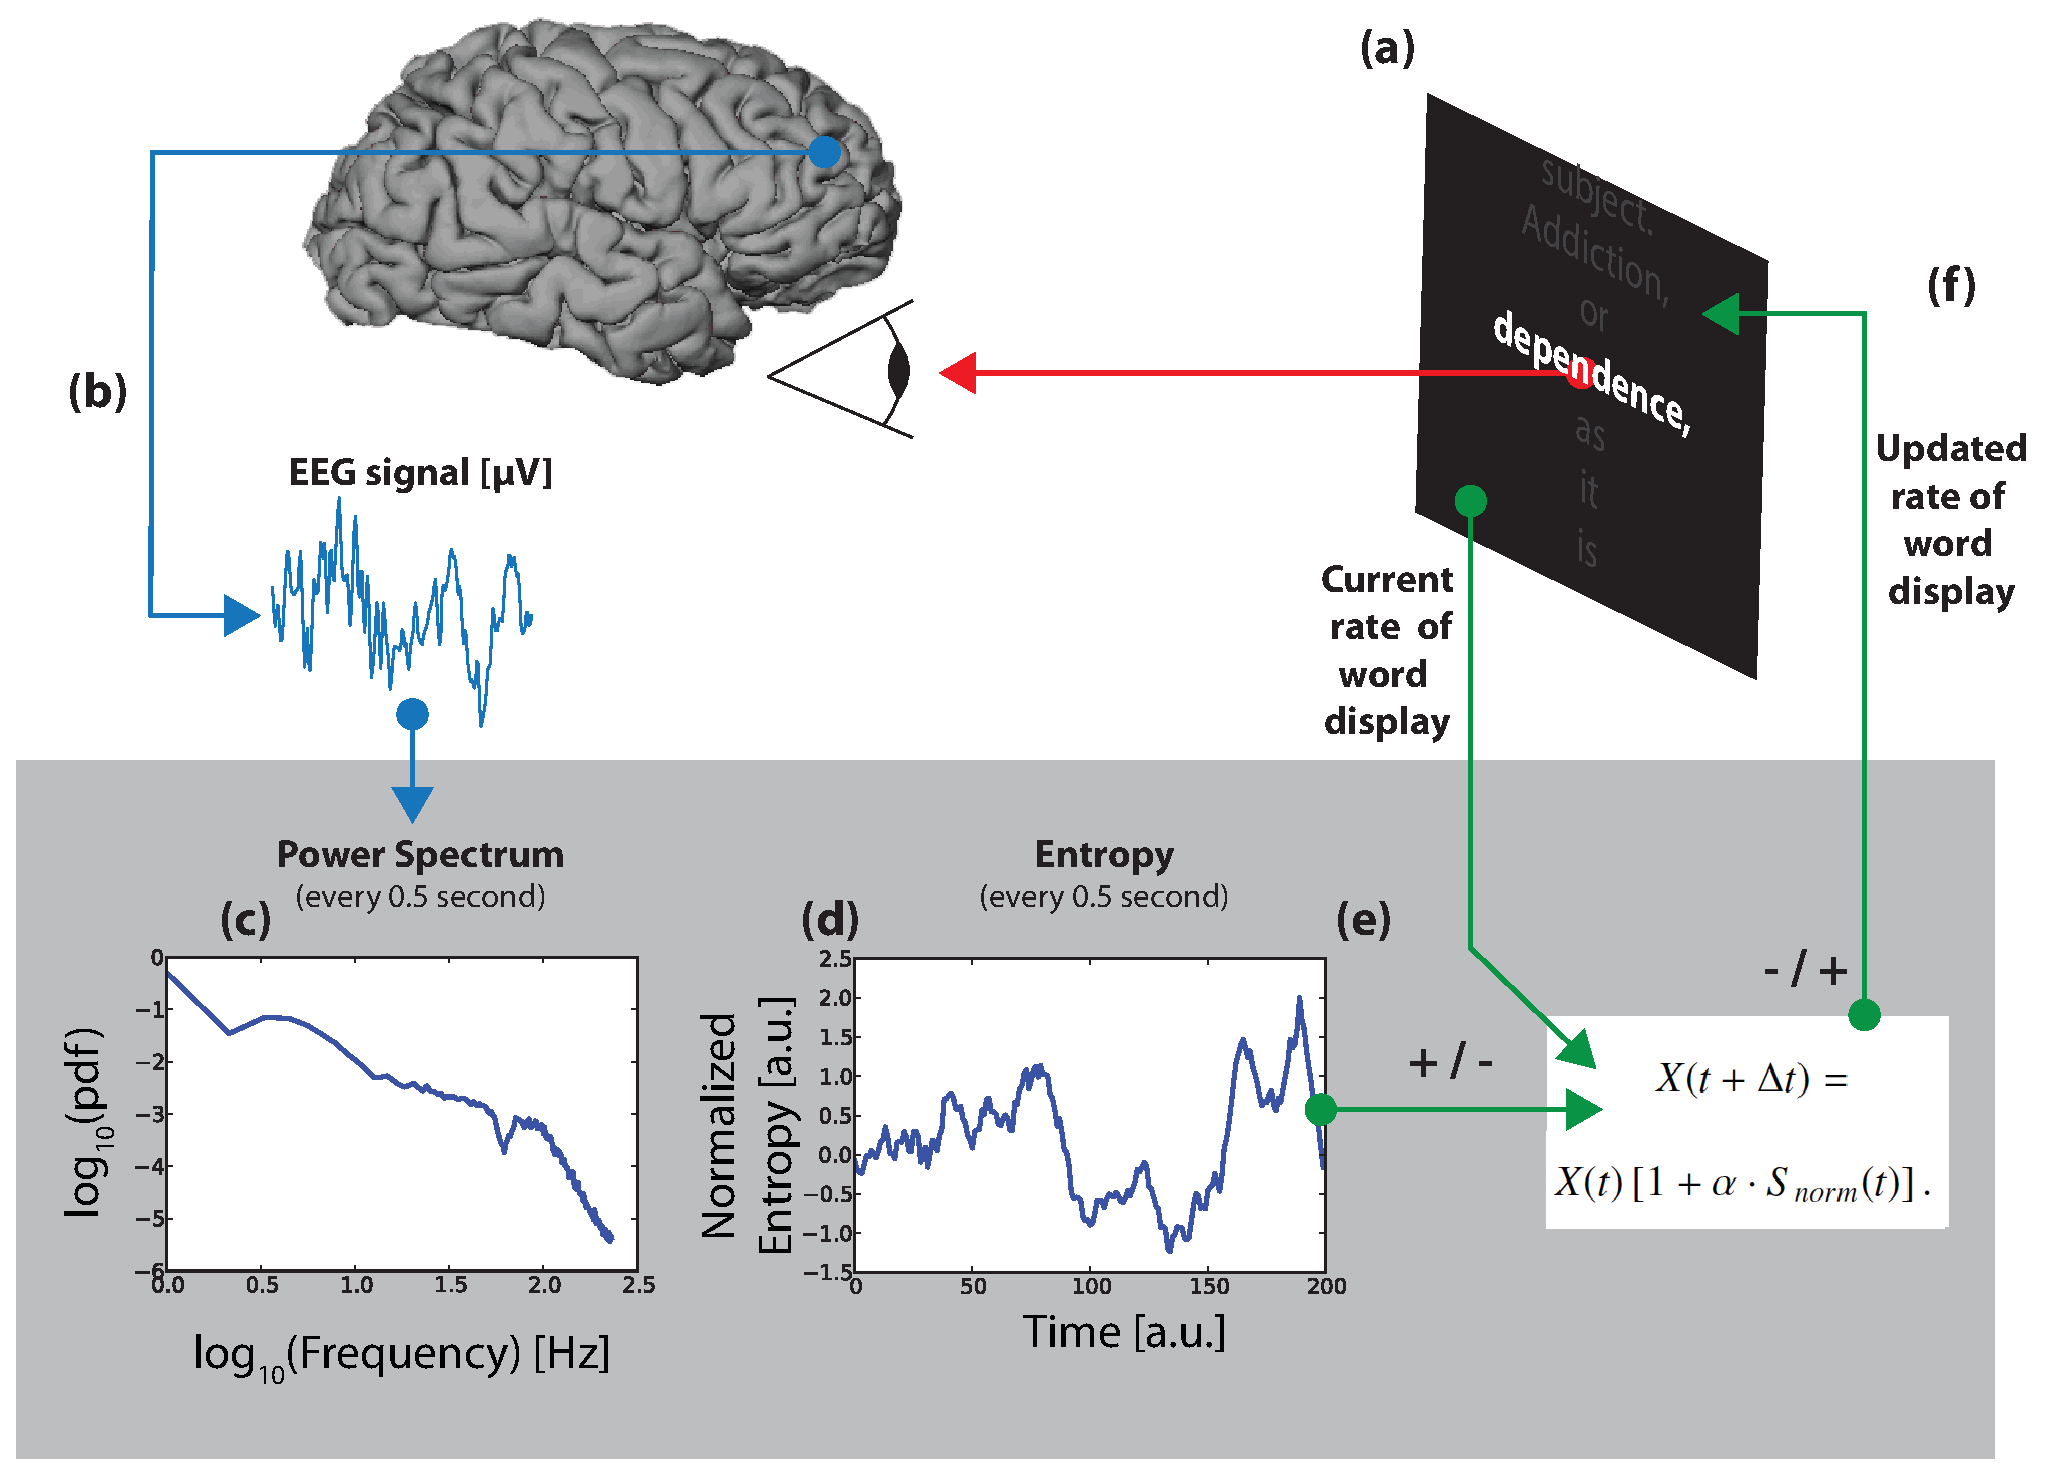
\includegraphics[width=7cm]{../figures2/apparatus.eps}
\caption{Brain speed-reader apparatus: {\bf (a)} Words are displayed and read one after the other at a given rate. {\bf (b)} the EEG signal is recorded through a consumer grade device (here the {\it Neurosky Mindwave}). {\bf (c)} The EEG signal is turned every 0.5 seconds into a power spectrum through a Fourier transform, {\bf (d)} the characteristics of the power spectrum are compressed into a single value characteristic entropy $s$ value. {\bf (e)} A new rate of word display is updated by taking into its current value and $s$. {\bf (f)} The rate of word display is updated accordingly.}
\label{fig:apparatus}
\end{figure}

\begin{figure}[H]
\centering
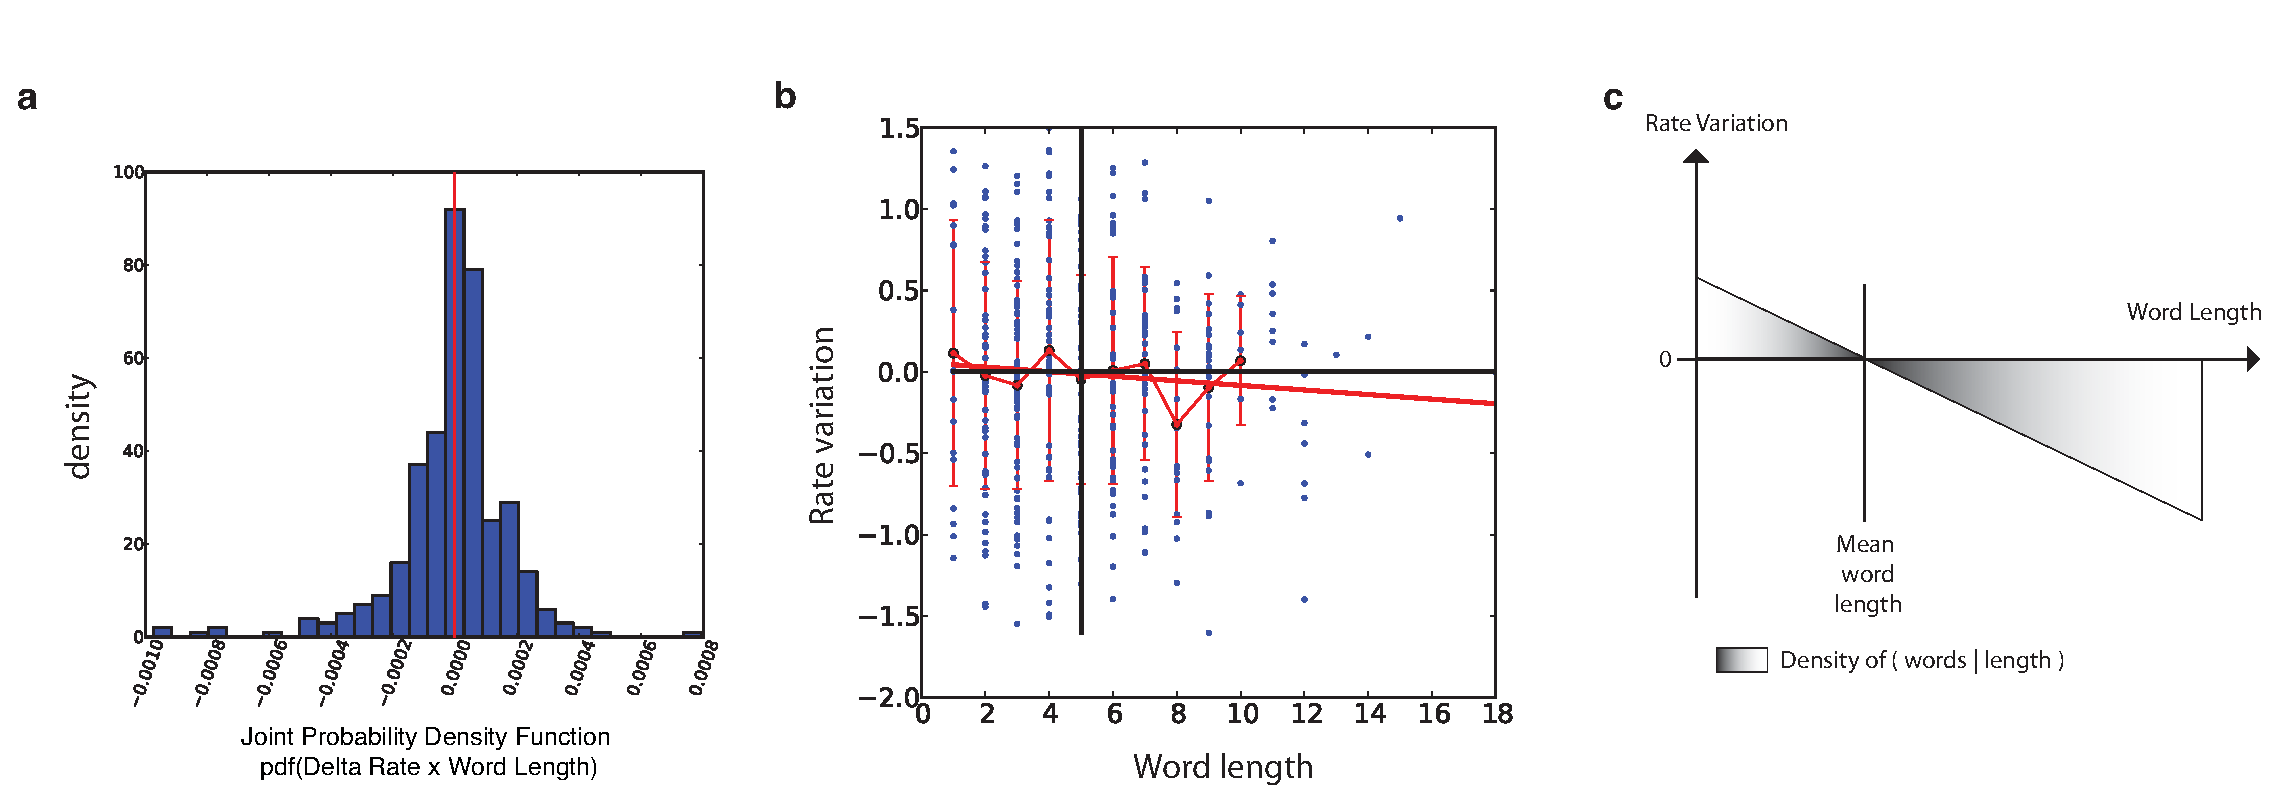
\includegraphics[width=17cm]{../figures2/balance.eps}
\caption{{\bf a.} Schematic representation of the balance of rate change $\Delta_{rate}$ as a function of word length $l_{words}$. The color gradient shows schematically the word density conditioned on their length. This is the canonical or most desirable situation: Around the mean word length the deterministic component of $\Delta_{rate}$ is close to zero. For words with length smaller, the deterministic part of the rate increases, while for words with length larger than the mean, the rate is decreased. The dotted line shows another possible configuration, with acceleration occurring when words are longer. Empirical evidence for the latter case is shown  in Figure \ref{fig:examples} for some typical successful and failed attempts to maintain a balance. ({\bf c}) The joint probability density function $pdf( \Delta_{rate} \times l_{words})$ is well balanced, yet skewed, showing that good control is achieved, along with a good capacity to change the rate of word display.}
\label{fig:apparatus}
\end{figure}

%The linear regression of the average $\Delta_{rates}$ for each word length (for $l_{words} < 10$) exhibits a slope $= 4(1)\times10^{-3}$ ($p < 0.01$). The intersection of $l_{words}(\Delta_{rates} =0) = 4.43$ very close to the average word length (in the text). The error bars show the dispersion (standard deviation of  $\Delta_{rates}$ for each word length. This dispersion is rather large reflecting the stochastic nature of complex brain activation sand the coarse measure obtained from the single electrode EEG headset.

\begin{figure}[H]
\centering
\includegraphics[width=12cm]{../figures2/examples.eps}
\caption{Four examples of successful and failed neuro-feedback control strategies. For each case, three panels are shown (from left to right): (i) Evolution of rate at each displayed word, (ii) rate change as a function of word length at each time step, and (iii)  rate change in the vicinity of large words (9 or more characters, red line), versus words with smaller than 5 characters (blue). The 90\% confidence intervals (light blue area) are obtained by replacement bootstrapping (100 samples of same size as large words are randomly drawn from small words). {\bf a.} Illustration of a very well controlled RSVP, with a sharp and localized drop of word presentation rate around the time large word occurrence. {\bf b.} Opposite strategy with rate increased around large words. {\bf c.} Yet another neuro-feedback strategy with the rate being controlled after the word has occurred. {\bf d.} Failed strategy: Compared to {\bf a}, {\bf b} and {\bf c} the rate change is consistently negative, hence dragging RSVP towards the lower rate limit. Note also in {\bf c} how the rate change as a function of word length (middle panel) is unbalanced around the 0-rate change (horizontal black line) and the mean word length (vertical black line), on the  contrary to {\bf a}, {\bf b} and {\bf c}.}
\label{fig:examples}
\end{figure}


\begin{figure}[H]
\centering
%\includegraphics[width=12cm]{../figures2/examples.eps}
\caption{Here a figure on how the rate is influenced by the power septrum. The idea is to cherry pick moments of high rate change, and look how the power spectrum (and entropy) influences these changes (keep in mind the smoothing, which should reduce the effects of pSpectrum changes on the rate.).}
\label{fig:S_vs_rate}
\end{figure}

\begin{figure}[H]
\centering
%\includegraphics[width=12cm]{../figures2/examples.eps}
\caption{To measure whether there is an effect in the constant rate case, one must first reverse engineer how the rate influences some power spectrum, and how it influences the rate}
\label{fig:constant_rate}
\end{figure}





%\section{Figures}

\begin{figure}[H]
\centering
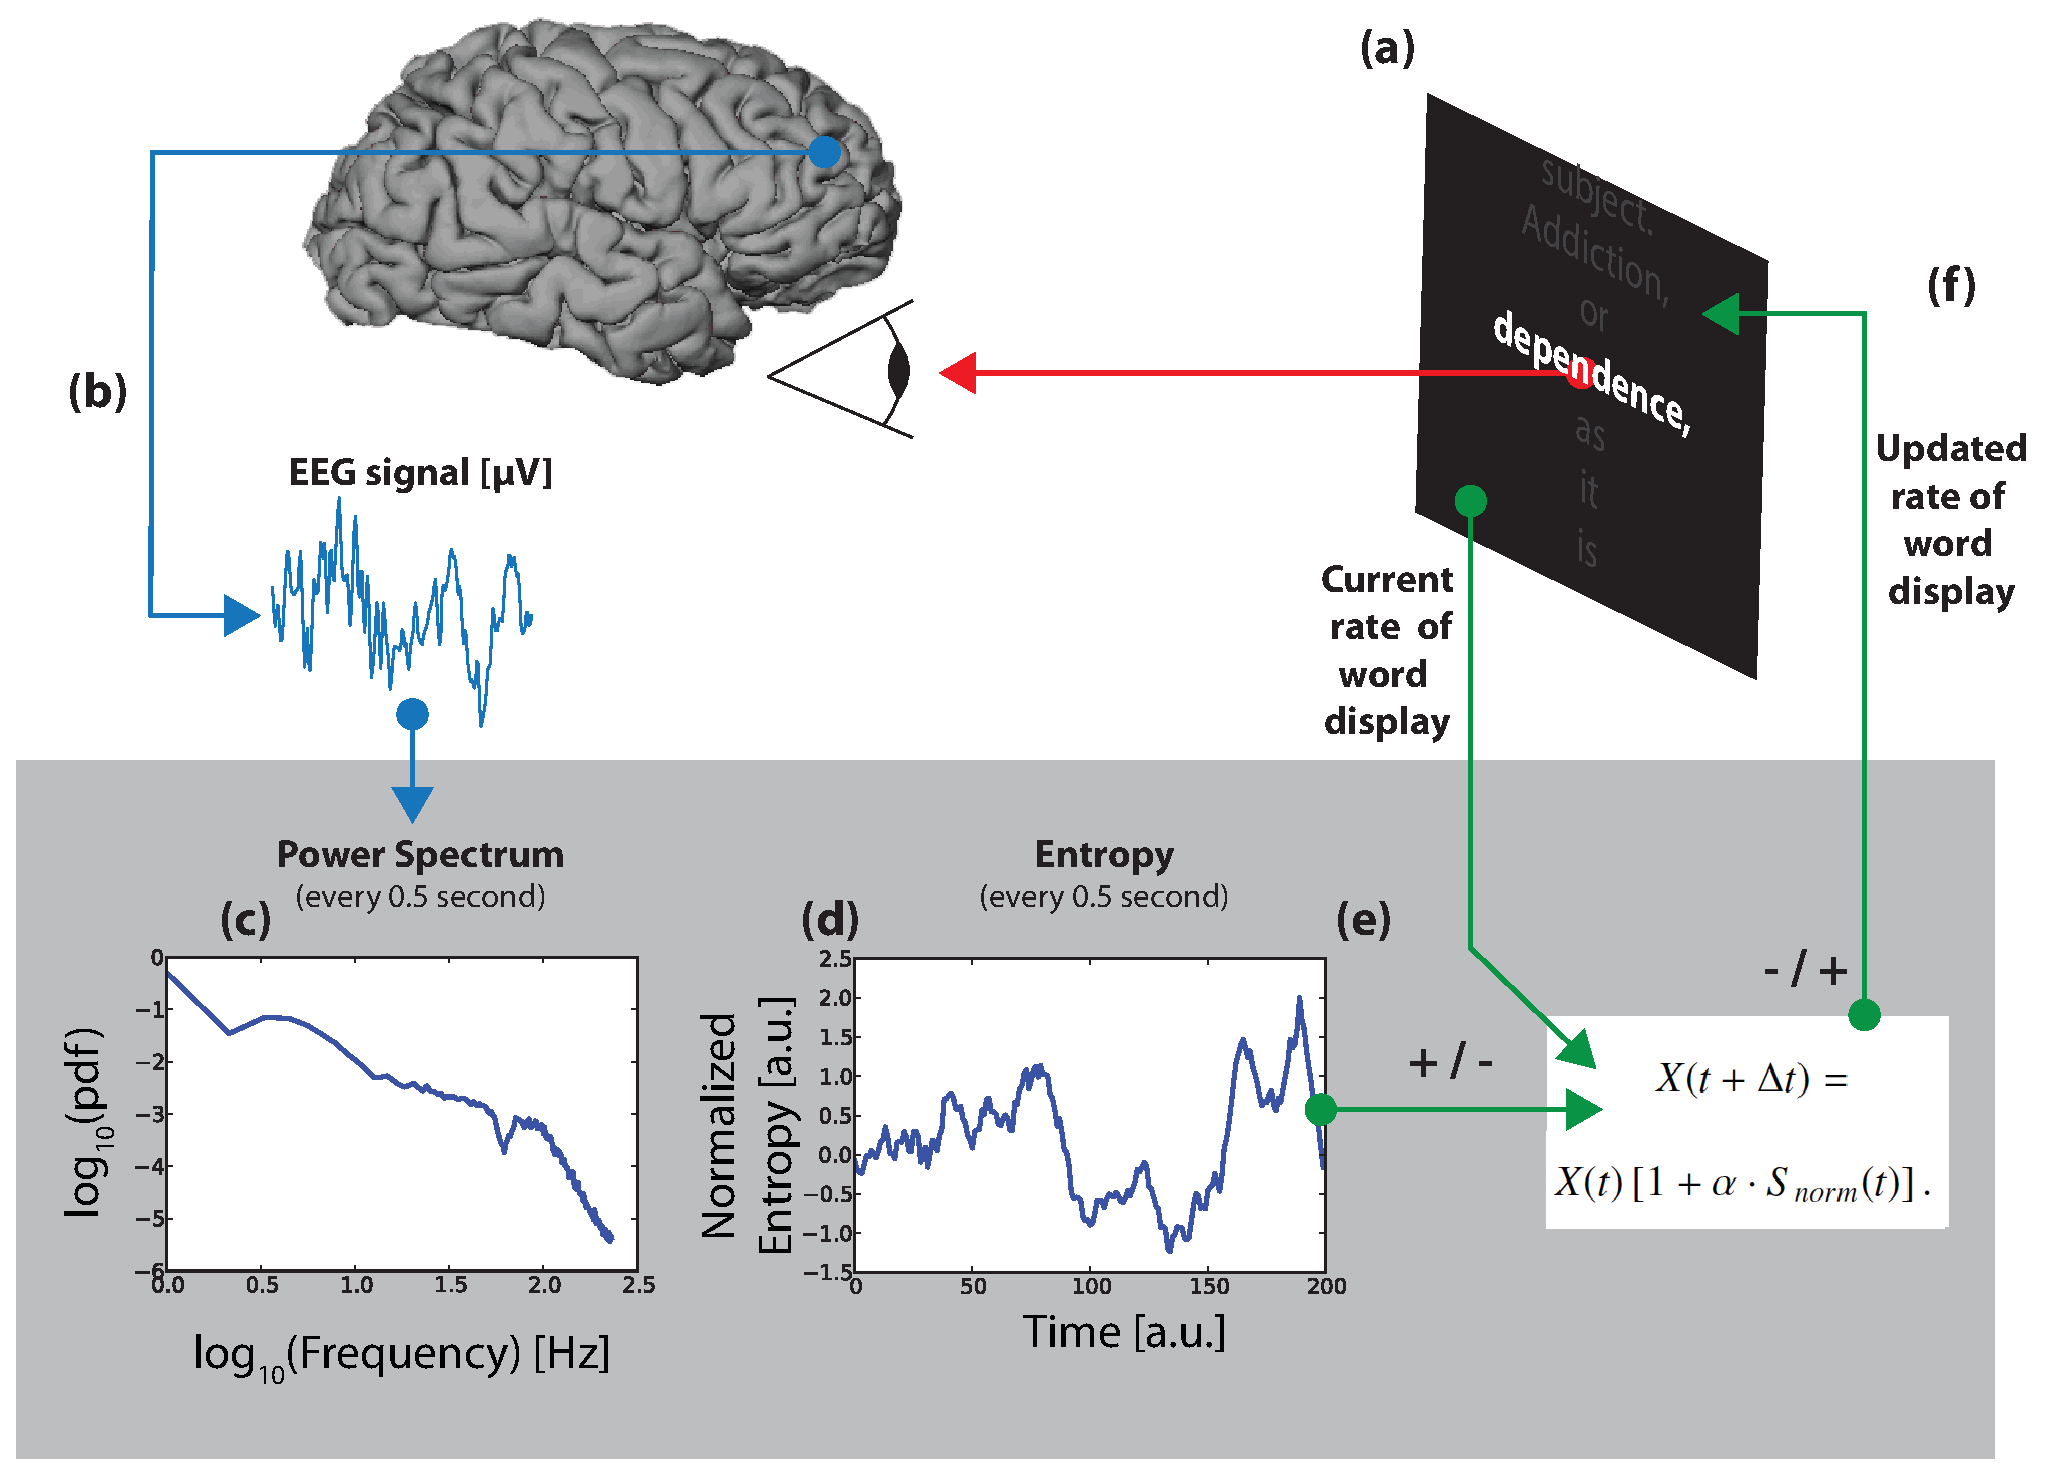
\includegraphics[width=7cm]{../figures2/apparatus.eps}
\caption{Brain speed-reader apparatus: {\bf (a)} Words are displayed and read one after the other at a given rate. {\bf (b)} the EEG signal is recorded through a consumer grade device (here the {\it Neurosky Mindwave}). {\bf (c)} The EEG signal is turned every 0.5 seconds into a power spectrum through a Fourier transform, {\bf (d)} the characteristics of the power spectrum are compressed into a single value characteristic entropy $s$ value. {\bf (e)} A new rate of word display is updated by taking into its current value and $s$. {\bf (f)} The rate of word display is updated accordingly.}
\label{fig:apparatus}
\end{figure}

\begin{figure}[H]
\centering
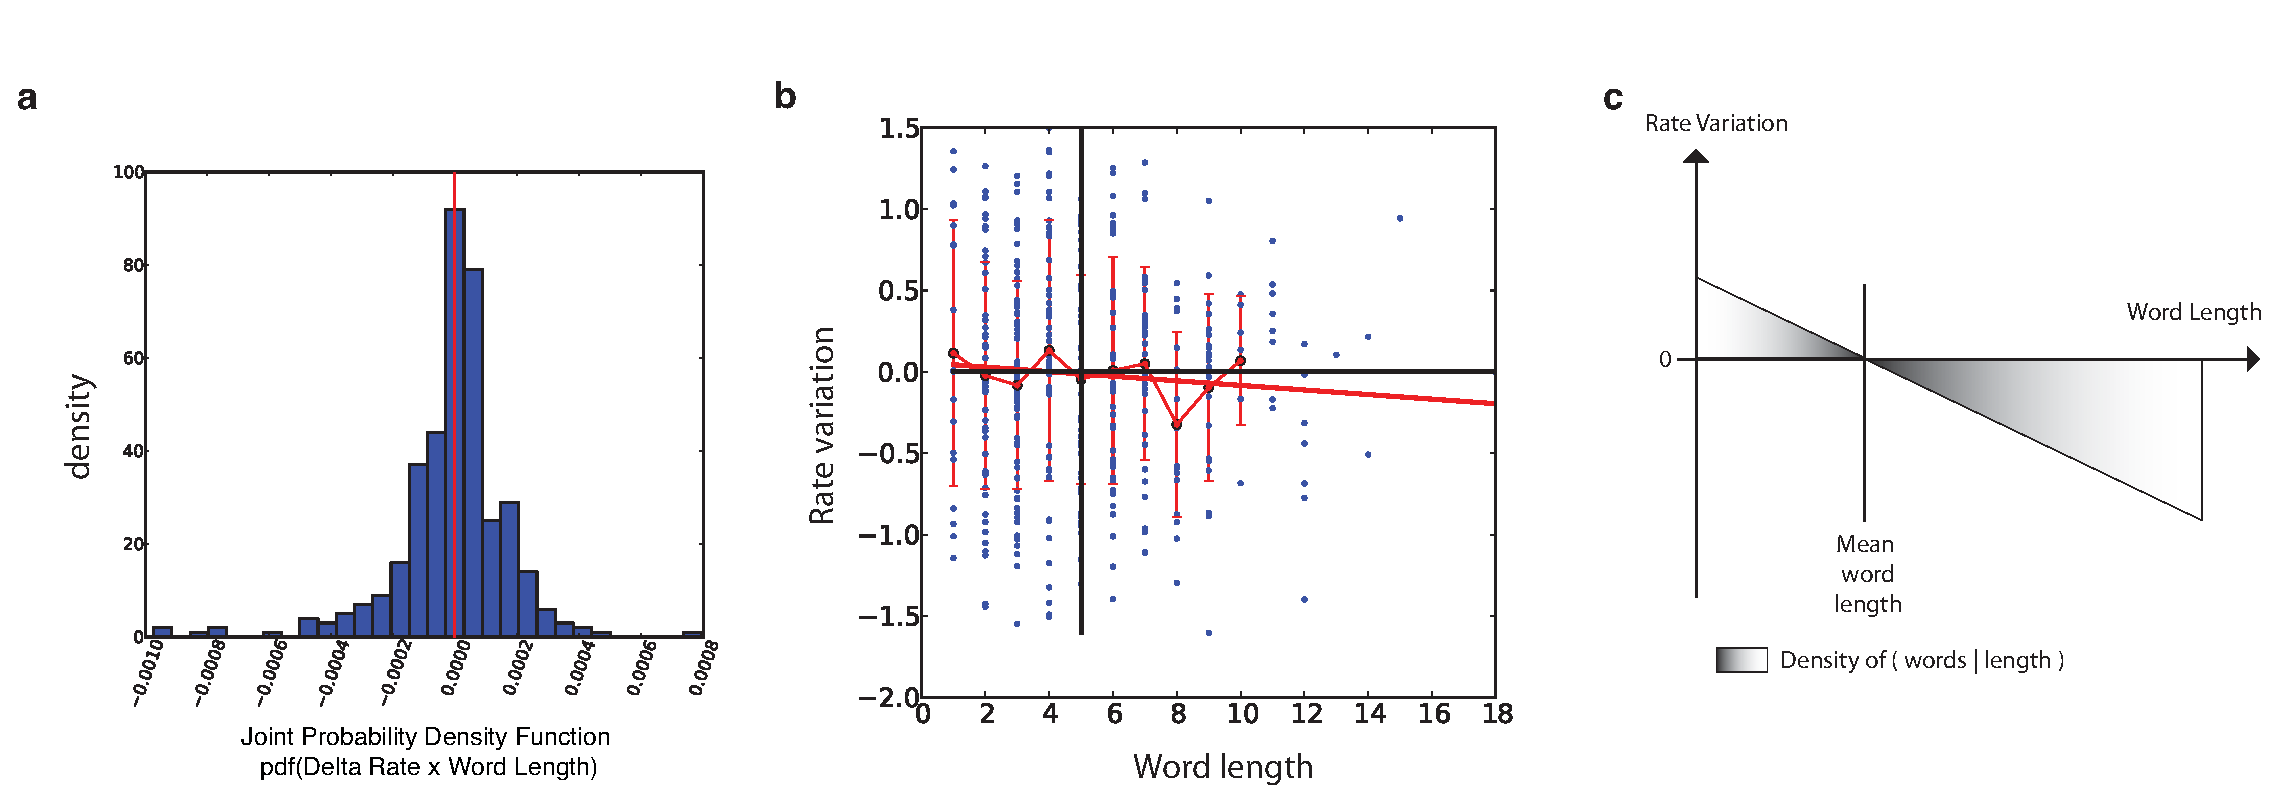
\includegraphics[width=17cm]{../figures2/balance.eps}
\caption{{\bf a.} Schematic representation of the balance of rate change $\Delta_{rate}$ as a function of word length $l_{words}$. The color gradient shows schematically the word density conditioned on their length. This is the canonical or most desirable situation: Around the mean word length the deterministic component of $\Delta_{rate}$ is close to zero. For words with length smaller, the deterministic part of the rate increases, while for words with length larger than the mean, the rate is decreased. The dotted line shows another possible configuration, with acceleration occurring when words are longer. Empirical evidence for the latter case is shown  in Figure \ref{fig:examples} for some typical successful and failed attempts to maintain a balance. ({\bf c}) The joint probability density function $pdf( \Delta_{rate} \times l_{words})$ is well balanced, yet skewed, showing that good control is achieved, along with a good capacity to change the rate of word display.}
\label{fig:apparatus}
\end{figure}

%The linear regression of the average $\Delta_{rates}$ for each word length (for $l_{words} < 10$) exhibits a slope $= 4(1)\times10^{-3}$ ($p < 0.01$). The intersection of $l_{words}(\Delta_{rates} =0) = 4.43$ very close to the average word length (in the text). The error bars show the dispersion (standard deviation of  $\Delta_{rates}$ for each word length. This dispersion is rather large reflecting the stochastic nature of complex brain activation sand the coarse measure obtained from the single electrode EEG headset.

\begin{figure}[H]
\centering
\includegraphics[width=12cm]{../figures2/examples.eps}
\caption{Four examples of successful and failed neuro-feedback control strategies. For each case, three panels are shown (from left to right): (i) Evolution of rate at each displayed word, (ii) rate change as a function of word length at each time step, and (iii)  rate change in the vicinity of large words (9 or more characters, red line), versus words with smaller than 5 characters (blue). The 90\% confidence intervals (light blue area) are obtained by replacement bootstrapping (100 samples of same size as large words are randomly drawn from small words). {\bf a.} Illustration of a very well controlled RSVP, with a sharp and localized drop of word presentation rate around the time large word occurrence. {\bf b.} Opposite strategy with rate increased around large words. {\bf c.} Yet another neuro-feedback strategy with the rate being controlled after the word has occurred. {\bf d.} Failed strategy: Compared to {\bf a}, {\bf b} and {\bf c} the rate change is consistently negative, hence dragging RSVP towards the lower rate limit. Note also in {\bf c} how the rate change as a function of word length (middle panel) is unbalanced around the 0-rate change (horizontal black line) and the mean word length (vertical black line), on the  contrary to {\bf a}, {\bf b} and {\bf c}.}
\label{fig:examples}
\end{figure}


\begin{figure}[H]
\centering
%\includegraphics[width=12cm]{../figures2/examples.eps}
\caption{Here a figure on how the rate is influenced by the power septrum. The idea is to cherry pick moments of high rate change, and look how the power spectrum (and entropy) influences these changes (keep in mind the smoothing, which should reduce the effects of pSpectrum changes on the rate.).}
\label{fig:S_vs_rate}
\end{figure}

\begin{figure}[H]
\centering
%\includegraphics[width=12cm]{../figures2/examples.eps}
\caption{To measure whether there is an effect in the constant rate case, one must first reverse engineer how the rate influences some power spectrum, and how it influences the rate}
\label{fig:constant_rate}
\end{figure}





%\setcounter{section}{0}
%\renewcommand\thesection{\Alph{section}}
%\renewcommand\thesubsection{\thesection.\arabic{subsection}}
%\renewcommand\thesubsubsection{\alph{subsubsection}}
%\clearpage
%\begin{center}
%{\bf \Huge Supplementary Materials}
%\end{center}
%\vspace{2cm}


%\section*{Tables}
%\begin{table}[!ht]
%\caption{
%\bf{Table title}}
%\begin{tabular}{|c|c|c|}
%table information
%\end{tabular}
%\begin{flushleft}Table caption
%\end{flushleft}
%\label{tab:label}
% \end{table}

\end{document}

